%Bojan nestorovic

\section{Deployment}

Postoje mnogi dodaci koji se koriste da prebace build fajlove posle uspesnog kompajliranja na željenu lokaciju ili web server. Ovde ćemo to pokazati na primeru "Deploy to container Plugin". 

\subsection{Instalacija dodatka Deploy to container Plugin}

Da bi se instalirao taj dodatak, potrebno je otići na Jenkins -> Manage Plugins, pronađete željeni dodatak i instalirate ga kao što je prikazano na slici \ref{fig:deploy_to_container_plugin}. Posle toga je potrebno restartovati jenkins server. Ovaj dodatak uzima fajlove i prebacuje ih automatski na server na kraju svakog builda.
\begin{figure}
\begin{center}
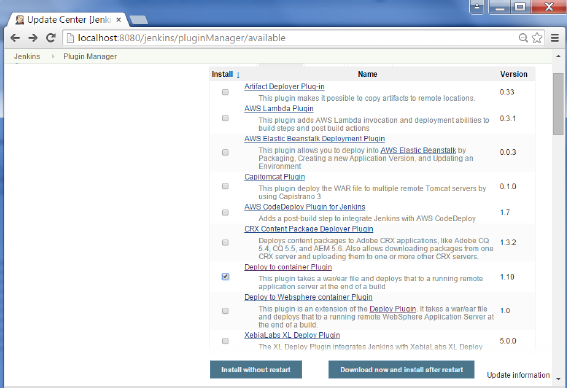
\includegraphics[scale=0.45]{slike/deploy_to_container_plugin.png}
\end{center}
\caption{Dodavanje dodatka}
\label{fig:deploy_to_container_plugin}
\end{figure}


\subsection{Podešavanje}

Potrebno je otići na Vaš Build project i kliknuti na Configure option. Izaberite opciju "Deploy war/ear to a container" kao što je prikazano na slici \ref{fig:deploy_war_ear_container}.

\begin{figure}
\begin{center}
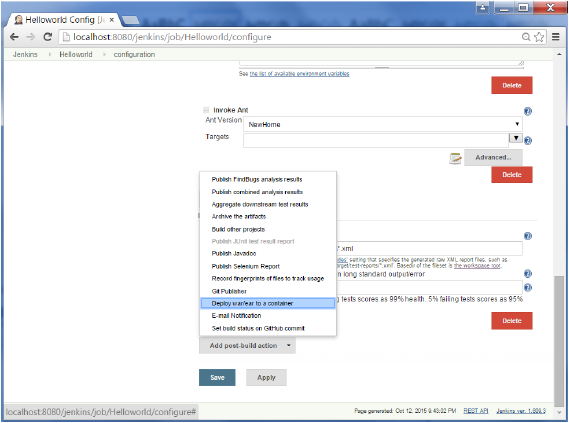
\includegraphics[scale=0.45]{slike/deploy_war_ear_container.png}
\end{center}
\caption{Deploy war/ear to a container dodatak}
\label{fig:deploy_war_ear_container}
\end{figure}

U polja prikazana na slici \ref{fig:demo_config.png} unesite detalje servera na kojem želite da se fajlovi šalju i kliknite na Save dugme. Ovi koraci će obezbediti da se potrebni fajlovi nadju na serveru posle uspešnog build-a.

\begin{figure}
\begin{center}
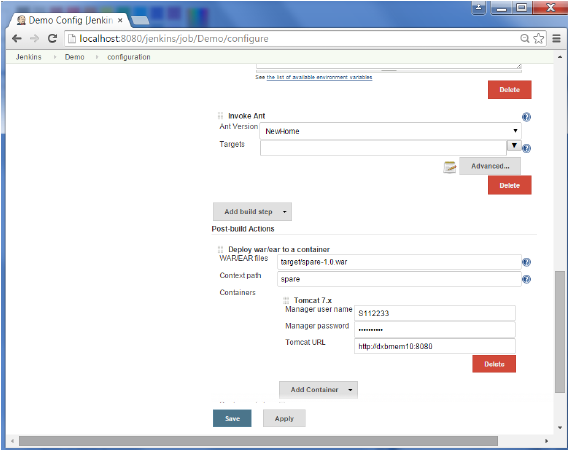
\includegraphics[scale=0.45]{slike/demo_config.png}
\end{center}
\caption{Konfigurisanje parametara}
\label{fig:demo_config.png}
\end{figure}


